% Dans l'introduction, on présente le problème étudié et les buts
% poursuivis. L'introduction permet de faire connaître le cadre de la
% recherche et d'en préciser le domaine d'application. Elle fournit
% les précisions nécessaires en ce qui concerne le contexte de
% réalisation de la recherche, l'approche envisagée, l'évolution de
% la réalisation. En fait, l'introduction présente au lecteur ce
% qu'il doit savoir pour comprendre la recherche et en connaître la
% portée.
\Chapter{INTRODUCTION}\label{sec:Introduction}  % 10-12 lignes pour introduire le sujet.

Les graphes de connaissance constituent l'ossature du Web sémantique, et trouvent aujourd'hui des applications toujours plus variées : ils servent pour la recherche d'information \cite{bounhas2019building, dietz2018utilizing}, la recommandation de contenu \cite{ying2018graph, wang2018ripplenet, wang2019explainable} ou la réponse automatique aux questions \cite{zhang2018variational, lukovnikov2017neural, saha2018complex}.  %
Au-delà de l'informatique, ils sont désormais utilisés dans des domaines aussi divers que les sciences biomédicales \cite{bakal2018exploiting, sousa2020evolving}, la recherche historique \cite{hyvonen2019knowledge, wilcke2017user} ou les sciences sociales \cite{heling2019building}.

%, mais aussi pour la recherche biomédicale \cite{bakal2018exploiting, sousa2020evolving}.
%
Un graphe de connaissance est constitué d'entités reliées les unes aux autres par des relations, mais aussi d'une ontologie, c'est-à-dire d'une collection d'axiomes logiques qui en décrit le contenu : ces axiomes définissent et caractérisent des classes (autrement dit, des groupes d'entités ayant des caractéristiques communes),  établissent des liens logiques entre classes, relations et entités et peuvent imposer des contraintes sur les données. Toutefois, si l'extraction automatique de graphes de connaissance à partir du Web est désormais courante \cite{auer2007dbpedia}, la création automatique d'ontologie demeure un problème ouvert. On introduit ici le contexte et les enjeux de ce problème, et les difficultés qui y sont liées.

% \clearpage

\section{Éléments de la problématique}  % environ 3 pages

%Un graphe de connaissance est principalement composé de trois types d'éléments : des éléments, des relations

Comme n'importe quelle base de données, un graphe de connaissance stocke de l'information de manière structurée et la rend accessible par le biais de requêtes; toutefois, contrairement aux bases de données relationnelles classiques, il ne nécessite pas de définir un schéma \textit{a priori} et une fois pour toutes. Cela facilite l'ajout de faits nouveaux, permet d'aggréger plus facilement des sources diverses et de lier des graphes de connaissance entre eux, ce qui constitue la clé du Web des données (\textit{Linked Data}).
Par rapport au texte, qui constitue un autre moyen dominant pour représenter la connaissance humaine, le graphe de connaissance présente l'avantage d'avoir une sémantique formelle, qui fournit une interprétation non-ambigüe des faits qu'il contient et permet donc son utilisation par des machines.
% et permet l'inférence de faits nouveaux.

Pour tirer pleinement profit de cette structure, il faut disposer d'une ontologie aussi complète que possible. %, c'est-à-dire d'un ensemble d'axiomes décrivant les données. La forme la plus simple d'un axiome relie simplement une entité à un ou plusieurs concepts
%
En effet, une ontologie permet la détection d'incohérences au sein d'un graphe \cite{inconsistencies2012dbpedia}, le typage automatique d'entités \cite{typing2017kejriwal} ou l'inférence de faits nouveaux \cite{inference2015dinto}. Les ontologies facilitent également la fusion de graphes de connaissance, c'est-à-dire la mise en correspondance de plusieurs graphes, grâce à des méthodes d'alignements \cite{otero2015ontology}. Dans le cas d'un graphe extrait automatiquement, une ontologie peut être utilisée pour l'extraction, le nettoyage ou l'uniformisation des données \cite{webmining2011bhatia, webmining2014li}. Les ontologies constituent également une piste prometteuse dans le domaine de l'intelligence artificelle explicable (\textit{explainable AI}) \cite{explainable2018holzinger, explainable2019cardillo, explainable2019semantic}.

Or construire une ontologie manuellement est coûteux, d'autant plus que la plupart des graphes sont dynamiques et changent au cours du temps : des nouvelles entités, relations, classes apparaissent; des axiomes qui étaient vrais ne le sont plus et inversement. L'ontologie doit changer elle aussi pour refléter ces changements. Dans ces conditions, pouvoir construire automatiquement une ontologie à partir du graphe est un enjeu important pour l'extraction et la maintenance automatique et à grande échelle de graphes de connaissance cite.

Le problème de l'extraction automatique d'ontologies est très étudié, et notamment sous une forme particulière : l'extraction de \textit{taxonomies}. Une taxonomie est une hiérarchie entre les classes d'un graphe; on peut la voir comme une ontologie réduite à des axiomes de la forme $A \sqsubset B$, qui indique que la classe $A$ est une sous-classe de $B$, et donc que toutes les entités qui font partie de $A$ font également partie de $B$. De tels axiomes sont appelés axiomes de \textit{subsumption}; un exemple de taxonomie est donné à la figure \ref{fig:intro-taxo}.

\begin{figure}[h]
    \centering
    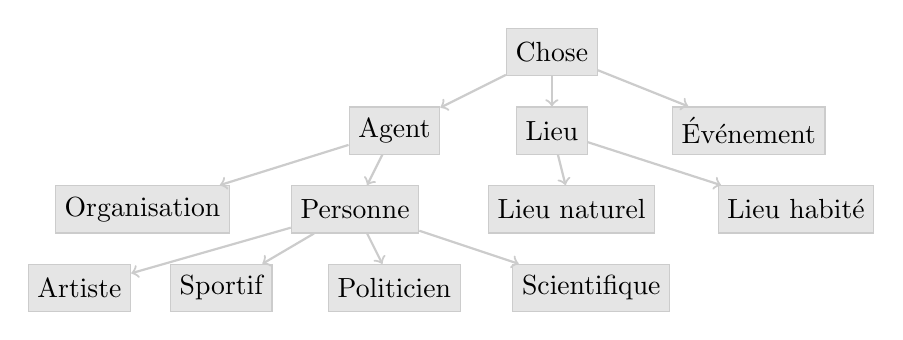
\begin{tikzpicture}[cnode/.style={draw=black,fill=#1,minimum width=3mm,circle},
    rnode/.style={draw=gray!40,fill=gray!20,minimum width=6mm, minimum height=6mm, rectangle}
]
    \node[rnode] (l11) at (0, 0) {Chose};
    \node[rnode] (l21) at (-2, -1) {Agent};
    \node[rnode] (l22) at (0, -1) {Lieu};
    \node[rnode] (l23) at (2.5, -1) {Événement};
    \node[rnode] (l31) at (-5.2, -2) {Organisation};
    \node[rnode] (l32) at (-2.5, -2) {Personne};
    \node[rnode] (l33) at (0.25, -2) {Lieu naturel};
    \node[rnode] (l34) at (3.1, -2) {Lieu habité};
    \node[rnode] (l41) at (-6, -3) {Artiste};
    \node[rnode] (l42) at (-4.2, -3) {Sportif};
    \node[rnode] (l43) at (-2, -3) {Politicien};
    \node[rnode] (l44) at (0.5, -3) {Scientifique};
    \draw[->, gray!40, thick] (l11) -- (l23);
    \draw[->, gray!40, thick] (l11) -- (l21);
    \draw[->, gray!40, thick] (l11) -- (l22);
    \draw[->, gray!40, thick] (l21) -- (l31);
    \draw[->, gray!40, thick] (l21) -- (l32);
    \draw[->, gray!40, thick] (l22) -- (l33);
    \draw[->, gray!40, thick] (l22) -- (l34);
    \draw[->, gray!40, thick] (l32) -- (l41);
    \draw[->, gray!40, thick] (l32) -- (l42);
    \draw[->, gray!40, thick] (l32) -- (l43);
    \draw[->, gray!40, thick] (l32) -- (l44);
\end{tikzpicture}


    \caption{Un exemple de taxonomie généraliste.}
    \label{fig:intro-taxo}
\end{figure}


Pour extraire une taxonomie, on peut s'appuyer sur le contenu d'un graphe de connaissance \cite{cimiano2004conceptual, zhang2019new, volker2011statistical, zhang2019iteratively, ristoski2017large} ou sur un corpus textuel
\cite{wu2008automatically, shwartz-etal-2017-hypernyms, fu2014learning, gupta2016domain, atzori2020fully, pocostales-2016-nuig}. Ce choix d'un graphe ou d'un corpus délimite deux grandes familles d'approches, qui utilisaient à l'origine des méthodes très différentes :
inférence de nouveaux axiomes par des méthodes symboliques ou statistiques dans le premier cas \cite{cimiano2004conceptual, volker2011statistical},  identification de motifs lexico-syntaxiques dans un texte dans le second cas \cite{hearst1992automatic, roller-etal-2018-hearst}. Aujourd'hui, 
on observe une certaine convergence des méthodes grâce à l'utilisation de représentations vectorielles denses des éléments manipulés (qu'il s'agisse d'entités ref, de mots \cite{mikolov2013distributed} ou de classes ref). Ces représentations vectorielles visent à traduire certaines régularités sous forme géométrique, afin que des éléments similaires (par exemple, des mots aux sens apparentés) soient représentés par des vecteurs géométriquement proches. Dans le cas d'un graphe, on parle de \textit{plongements vectoriels de graphe} (ou \textit{knowledge graph embeddings} en anglais); dans le cas du texte, on parle de \textit{plongements lexicaux} (ou \textit{word embeddings} en anglais). Un exemple de tels plongements est représenté à la figure \ref{fig:intro-embeddings}.

%
% illu (PCA of word and graph embeddings FastText/TransE)

\begin{figure}[h]
    \centering
    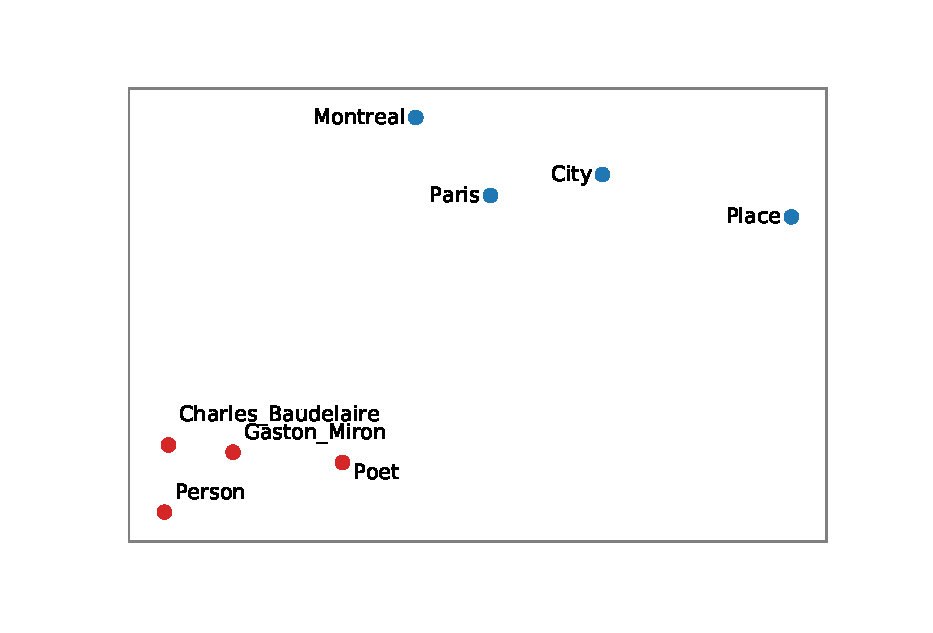
\includegraphics[width=0.7\textwidth]{img/embedding_pca_transe2.eps}
    \caption[Exemple de plongements vectoriels]{
    Un exemple de plongements vectoriels de graphe, représentés en deux dimensions\footnotemark.}
    \label{fig:intro-embeddings}
\end{figure}

\footnotetext{Ces plongements ont été obtenus sur DBpedia avec le modèle TransE. Leur dimension est ramenée de $d=50$ à $d=2$ grâce à une PCA.}

Qu'ils soient entraînés sur un graphe ou sur du texte, ces plongements permettent l'application de diverses techniques issues de l'apprentissage automatique au problème de l'extraction de taxonomie, par exemple en entraînant un classificateur capable de détecter la subsumption \cite{fu2014learning}, ou en regroupant les plongements sur la base de leur proximité géométrique \cite{gupta2016domain, zhang2018taxogen}.


Toutefois, la plupart de ces méthodes se contentent d'organiser hiérarchiquement des classes pré-existantes, et ne sont pas capables de caractériser ces classes (que ce soit au moyen d'axiomes logiques, de descriptions textuelles ou même de mots-clés), ni d'identifier de nouvelles classes à partir des données.
%
Dans le présent mémoire, nous proposons au contraire une identification non-supervisée de groupes d'entités cohérents, ce qui permet à la fois de détecter des classes, nouvelles ou pré-existantes, et de les organiser hiérarchiquement au sein d'une taxonomie. % Couplée à un algorithme d'extraction d'axiome, cette méthode permet 

% Nous montrons d'abord que cette identification non-supervisée est capable de reconstituer une taxonomie sur les classes existantes (c'est le cas non-expressif, décrit au chapitre \ref{chap:te}), puis nous l'utilisons pour extraire de nouvelles classes et les décrire au moyen d'axiomes logiques (c'est le cas expressif, décrit au chapitre \ref{chap:texp}).

% Dans ce travail, nous proposons une identification non-supervisée de groupes d'entités cohérents et pertinents, qui se décline en (a) une variante non-expressive, réclamant peu de données en entrée et (b) une variante expressive, qui utilise tout le graphe de connaissances et permet d'organiser hiérarchiquement les classes entre elles, de décrire les classes existantes au moyen d'axiomes logiques, et d'identifier de nouvelles classes à partir des données.


%%
%% OBJECTIFS DE RECHERCHE / RESEARCH OBJECTIVES
%%
\section{Objectifs de recherche}  % 0.5 page

Dans ce mémoire, nous cherchons à extraire une taxonomie expressive à partir des plongements vectoriels d'un graphe de connaissance.
%
Notre hypothèse est en effet que les plongements vectoriels intègrent dans leur géométrie des notions de proximité entre entités, mais aussi des informations de nature taxonomique, et
%
qu'il doit donc être possible de les utiliser à la fois pour l'identification de groupes d'entités et pour la hiérarchisation de ces groupes. 
%
Notre question de recherche s'énonce donc ainsi :

\begin{quote}
    \emph{Comment les plongements vectoriels de graphe peuvent-ils contribuer à l'extraction de taxonomie ?}
\end{quote}




Pour résoudre ce problème, nous proposons d'utiliser un regroupement hiérachique non-supervisé sur les plongements vectoriels, ce qui permet de créer une structure hiérarchique sur des groupes d'entités. Pour transformer cette structure en une taxonomie expressive ou non-expressive, il est nécessaire de répondre aux sous-questions suivantes :
%
%ce qui suppose de répondre aux sous-questions suivantes :
\begin{quote}
    \emph{\textbf{Q1.} Comment assigner des concepts à des groupes d'entités en tenant compte de la structure d'arbre entre ces groupes ?}
\end{quote}

\begin{quote}
    \emph{\textbf{Q2.} Comment décrire un groupe d'entités à l'aide d'axiomes logiques expressifs ?}
\end{quote}







%%
%% PLAN DU MEMOIRE / THESIS OUTLINE
%%
\section{Plan du mémoire}  % 0.5 page


% On présente d'abord une panorama de la littérature existante. Y sont introduits les concepts fondamentaux du Web sémantique : les graphes de connaissance, qui permettent une représentation structurée de la connaissance, et la logique descriptive, qui permet d'enrichir ces graphes de règles logiques dont la somme constitue une taxonomie ou une ontologie, selon leur complexité. On décrit ensuite les techniques existantes pour extraire automatiquement ces taxonomies, soit à partir d'un graphe, soit à partir de corpus textuels. On propose finalement un survol des méthodes pour inférer de nouveaux axiomes à partir d'un graphe.

On présente d'abord un panorama de la littérature existante au chapitre \ref{chap:revue}. On y introduit les concepts fondamentaux du Web sémantique, et notamment la logique descriptive. On décrit ensuite les techniques existantes pour extraire automatiquement des ontologies ou des taxonomies, que ce soit à partir de textes ou de graphes.

Le chapitre \ref{chap:kge} est consacré aux modèles de plongement, qui permettent une représentation vectorielle des éléments d'un graphe et servent de base à notre travail. On présente plusieurs familles de modèles, et on propose une méthode pour l'évaluation de ces modèles.


% On présente différents modèles concurrents, en s'efforçant de dégager les intuitions et les hypothèses qui ont dirigé leur conception, et de mettre en évidence leurs limitations théoriques et pratiques. On définit ensuite une nouvelle tâche pour l'évaluation de ces modèles, et on présente les résultats de cette évaluation.


% Dans le chapitre \ref{chap:te}, nous présentons une nouvelle approche pour extraire automatiquement  que 

Les deux chapitres suivants sont consacrés à notre méthodologie d'extraction de taxonomie à partir de graphes. Nous montrons que le regroupement non-supervisée de plongements vectoriels peut servir à reconstituer une taxonomie sur les classes existantes (chapitre \ref{chap:te}). Pour cela, nous proposons deux méthodes pour assigner un type à des groupes qui émergent d'un processus de regroupement hiérarchique.



Enfin, nous montrons que le regroupement non-supervisé permet également d'identifier de nouvelles classes, et donc de produire une taxonomie expressive : 
, %
et qu'il permet de surcroît d'identifier de nouvelles classes, et donc de produire une taxonomie expressive à partir du graphe (chapitre \ref{chap:texp}).

%puis nous l'utilisons pour extraire de nouvelles classes et les décrire au moyen d'axiomes logiques (c'est le cas expressif, décrit au chapitre \ref{chap:texp}).


% on présente une nouvelle approche pour extraire automatiquement une taxonomie à partir des plongements d'un graphe de connaissance. Le chapitre \ref{chap:texp} applique certaines des idées précédentes à l'extraction d'une taxonomie expressive. 
\clearpage